\section{Inteligência Artificial}

O termo aprendizado de máquina refere-se à detecção automatizada de padrões significantes em dados. Nas últimas décadas tem se tornado uma ferramenta comum em quase qualquer tarefa que requer informações extraídas de uma grande quantidade de dados \cite{uml}.

A ciência do aprendizado tem um importante papel em áreas como a estatística, mineração de dados e inteligência artificial, passando por áreas como engenharia, medicina, astronomia, robótica e outras disciplinas \cite{statistical-learning}.

Com o contínuo aumento de informações em forma digital, a necessidade de métodos automatizados para análise de dados continua crescendo. O objetivo do aprendizado de máquina é desenvolver métodos que possibilitam a detecção de padrões em dados, para futuramente reutilizá-los em forma de previsões em novos dados \cite{mlpp}. 

Dentre as ferramentas que integram a inteligência artificial destacam-se os Algoritmos Genéticos, Lógica Difusa e Redes Neurais Artificiais \cite{ai-fili}, sendo este trabalho focado em Redes Neurais Artificiais (RNA). A Figura \ref{fig:rede-neural} mostra um exemplo de rede artifical.

\begin{figure}[h]
    \caption{Exemplificação de uma rede neural artificial}
    \centering
    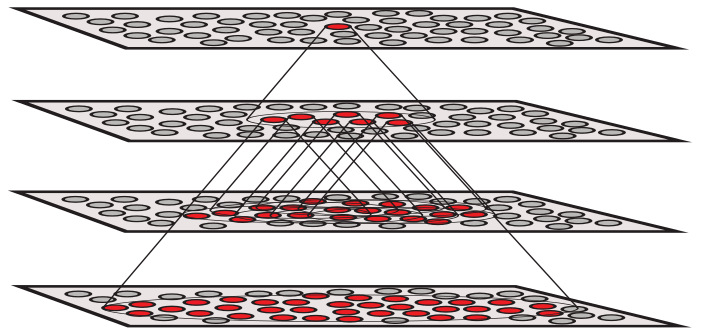
\includegraphics[width=0.8\textwidth]{Textuais/Figuras/supervi.png}
    \fonte{https://lamfo-unb.github.io/2017/07/27/tres-tipos-am}
    \label{fig:rede-neural}
\end{figure}